%%
%% Automatically generated file from DocOnce source
%% (https://github.com/hplgit/doconce/)
%%
%%


%-------------------- begin preamble ----------------------

\documentclass[%
oneside,                 % oneside: electronic viewing, twoside: printing
final,                   % draft: marks overfull hboxes, figures with paths
10pt]{article}

\listfiles               %  print all files needed to compile this document

\usepackage{relsize,makeidx,color,setspace,amsmath,amsfonts,amssymb}
\usepackage[table]{xcolor}
\usepackage{bm,ltablex,microtype}

\usepackage[pdftex]{graphicx}

\usepackage[T1]{fontenc}
%\usepackage[latin1]{inputenc}
\usepackage{ucs}
\usepackage[utf8x]{inputenc}

\usepackage{lmodern}         % Latin Modern fonts derived from Computer Modern

% Hyperlinks in PDF:
\definecolor{linkcolor}{rgb}{0,0,0.4}
\usepackage{hyperref}
\hypersetup{
    breaklinks=true,
    colorlinks=true,
    linkcolor=linkcolor,
    urlcolor=linkcolor,
    citecolor=black,
    filecolor=black,
    %filecolor=blue,
    pdfmenubar=true,
    pdftoolbar=true,
    bookmarksdepth=3   % Uncomment (and tweak) for PDF bookmarks with more levels than the TOC
    }
%\hyperbaseurl{}   % hyperlinks are relative to this root

\setcounter{tocdepth}{2}  % levels in table of contents

% Tricks for having figures close to where they are defined:
% 1. define less restrictive rules for where to put figures
\setcounter{topnumber}{2}
\setcounter{bottomnumber}{2}
\setcounter{totalnumber}{4}
\renewcommand{\topfraction}{0.95}
\renewcommand{\bottomfraction}{0.95}
\renewcommand{\textfraction}{0}
\renewcommand{\floatpagefraction}{0.75}
% floatpagefraction must always be less than topfraction!
% 2. ensure all figures are flushed before next section
\usepackage[section]{placeins}
% 3. enable begin{figure}[H] (often leads to ugly pagebreaks)
%\usepackage{float}\restylefloat{figure}

% prevent orhpans and widows
\clubpenalty = 10000
\widowpenalty = 10000

\newenvironment{doconceexercise}{}{}
\newcounter{doconceexercisecounter}


% ------ header in subexercises ------
%\newcommand{\subex}[1]{\paragraph{#1}}
%\newcommand{\subex}[1]{\par\vspace{1.7mm}\noindent{\bf #1}\ \ }
\makeatletter
% 1.5ex is the spacing above the header, 0.5em the spacing after subex title
\newcommand\subex{\@startsection*{paragraph}{4}{\z@}%
                  {1.5ex\@plus1ex \@minus.2ex}%
                  {-0.5em}%
                  {\normalfont\normalsize\bfseries}}
\makeatother


% --- end of standard preamble for documents ---


% insert custom LaTeX commands...

\raggedbottom
\makeindex
\usepackage[totoc]{idxlayout}   % for index in the toc
\usepackage[nottoc]{tocbibind}  % for references/bibliography in the toc

%-------------------- end preamble ----------------------

\begin{document}

% matching end for #ifdef PREAMBLE

\newcommand{\exercisesection}[1]{\subsection*{#1}}

% This file is to be run by preprocess to produce newcommands.tex
% to be included in .tex files.
% There are format-specific tests here for the newcommands (i.e.,
% different definitions of the commands depending on latex or mathjax).

% Newcommands for LaTeX math.
\newcommand{\tp}{\thinspace .}
\renewcommand{\Re}{\bbbr}
\newcommand{\Oof}[1]{\mathcal{O}(#1)}
\newcommand{\Prob}[1]{\hbox{P}(#1)}
\newcommand{\Var}[1]{\hbox{Var}(#1)}
\newcommand{\Cov}[2]{\hbox{Cov}(#1,#2)}
\newcommand{\StDev}[1]{\hbox{StDev}(#1)}

\newcommand{\punkt}{\thinspace .}
\newcommand{\komma}{\thinspace ,}

\newcommand{\vr}{\vec{r}}
\newcommand{\vrp}{\vec{r}\,'}
\newcommand{\erf}{\mathrm{erf}}
\newcommand{\vrho}{\vec{\varrho}}
\newcommand{\vrhop}{\vec{\varrho}\, '}
\newcommand{\sign}{\mathrm{sign}}

\newcommand{\Tr}[1]{\mathrm{Tr}[#1]}
\newcommand{\e}{\varepsilon}
\newcommand{\g}{\gamma}

\newcommand{\half}{\frac{1}{2}}
\newcommand{\vnabla}{\vec{\nabla}}


% Use footnotesize in subscripts
\newcommand{\subsc}[2]{#1_{\mbox{\footnotesize #2}}}




% ------------------- main content ----------------------



% ----------------- title -------------------------

\thispagestyle{empty}

\begin{center}
{\LARGE\bf
\begin{spacing}{1.25}
FFM234, Klassisk fysik och vektorfält - Veckans tal
\end{spacing}
}
\end{center}

% ----------------- author(s) -------------------------

\begin{center}
{\bf \href{{http://fy.chalmers.se/subatom/nt/}}{Christian Forssén}, Institutionen för fysik, Chalmers${}^{}$} \\ [0mm]
\end{center}

\begin{center}
% List of all institutions:
\end{center}
    
% ----------------- end author(s) -------------------------

% --- begin date ---
\begin{center}
Aug 10, 2019
\end{center}
% --- end date ---

\vspace{1cm}


% --- begin exercise ---
\begin{doconceexercise}
\refstepcounter{doconceexercisecounter}

\subsection*{Tentatal 2012-10-23: 6}

En punktladdning $Q$ är belägen i $\vec{r} = b\hat{z}$, och man söker potentialen från denna laddning innanför sfären $r = a$ (med $a > b$), då randvillkoret är att den elektriska potentialen $\phi$ är noll på randen $r = a$. 
\begin{itemize}
\item Visa att denna potential fås genom att introducera en fiktiv spegelladdning $−\frac{a}{b}Q$ i punkten $\vec{r} = \frac{a^2}{b} \hat{z}$. 

\item Ge ett uttryck för den ytladdningsfördelning som induceras på sfären $r = a$, om man antar att $\phi = 0$ även för $r > a$. 

\item Kontrollera att den totala inducerade laddningen på sfären är $−Q$.
\end{itemize}

\noindent
% --- begin hint in exercise ---

\paragraph{Hint.}
\begin{itemize}
\item Man kan direkt teckna potentialen som en superposition av potentialer från två punktladdningar, den verkliga i $b\hat{z}$ plus spegelladdningen enligt uppgiften. Glöm inte $1/\epsilon_0$. Kontrollera att denna potential uppfyller randvilloret.

\item Men det är en nyttig övning att gå hela vägen från Greensfunktionen (inklusive spegelladdning) och utföra volymsintegralen över sfären, där laddningstätheten ges av en deltafunktion $\rho(\vec{r}{\;}') = Q \delta^3(\vec{r}{\;}' - b\hat{z})$.

\item Ytladdningsfördelningen ges av $\epsilon_0 \left. \hat{r} \cdot \left( \vec{E}^+ - \vec{E}^- \right)  \right|_{r=a}$, där det elektriska fältet är $\vec{E} = - \nabla \phi$.

\item Totala inducerade laddningen på ytan fås genom att integrera över sfärens yta.
\end{itemize}

\noindent
% --- end hint in exercise ---


% --- begin answer of exercise ---
\paragraph{Answer.}
Ytladdningsfördelningen blir
$$
\sigma = -\frac{Q}{4 \pi} \frac{a^2 - b^2}{a \left( a^2 + b^2 - 2 a b \cos\theta \right)^{3/2}}
$$
Notera gärna att enheten blir lika med laddning per areaenhet, precis som den skall.

% --- end answer of exercise ---


% --- begin solution of exercise ---
\paragraph{Solution.}
Potentialen kan vi egentligen teckna direkt; dvs utan att skriva ner Greensfunktionen och utföra integralen. Med två punktladdningar på $z$-axeln, enligt uppgiften, och avstånd till dessa som fås med cosinussatsen (se figur nedan), blir potentialen lika med (glöm inte $1/\epsilon_0$)
$$
\phi(\vec{r}) = \frac{Q}{4\pi\epsilon_0} \left[ \frac{1}{\sqrt{r^2 + b^2 - 2 b r \cos\theta}} - \frac{a}{b} \frac{1}{\sqrt{r^2 + \frac{a^4}{b^2} - 2 \frac{a^2}{b} r\cos\theta}}\right].
$$
Men för att vara noggranna räknar vi ut ovanstående med hjälp av Greensfunktioner. Enligt uppgiftstexten skall spegelladdningar införas så att för en punktladdning i punkten $\vec{r}{\;}'$ skall det finnas en spegelladdning med styrkan $-a/r'$ i punkten $\vec{r}{\;}''$, där $\vec{r}{\;}'' = \frac{a^2}{(r')^2} \vec{r}{\;}'$. Greensfunktionen blir alltså
$$
G(\vec{r},\vec{r}{\;}') = \frac{1}{4\pi|\vec{r} - \vec{r}{\;}'|} - \frac{a}{r'} \frac{1}{4\pi|\vec{r} - \vec{r}{\;}''|},
$$
och den slutliga lösningen fås genom att integrera
$$
\phi(\vec{r}) = \frac{1}{\epsilon_0} \int_{V'} \mbox{d}V' \rho(\vec{r}{\;}') G(\vec{r},\vec{r}{\;}'),
$$
där volymen $V'$ alltså är sfären och laddningsfördelningen i vårt fall är en punktladdning med styrkan $Q$ i punkten $b\hat{z}$, dvs
$$
\rho(\vec{r}{\;}') = Q \delta^3(\vec{r}{\;}' - b\hat{z}).
$$
Integralen blir
$$
\phi(\vec{r}) = \frac{1}{\epsilon_0} \int_{V'} \mbox{d}V' \rho(\vec{r}{\;}') G(\vec{r},\vec{r}{\;}')
= \frac{Q}{4\pi\epsilon_0} \left[ \frac{1}{|\vec{r} - b\hat{z}|} - \frac{a}{b} \frac{1}{\left| \vec{r} - \frac{a^2}{b}\hat{z} \right|} \right],
$$
där vi använt att $\vec{r}{\;}'' = \frac{a^2}{b}\hat{z}$ när $\vec{r}{\;}'=b\hat{z}$.



\vspace{6mm}

% inline figure
\centerline{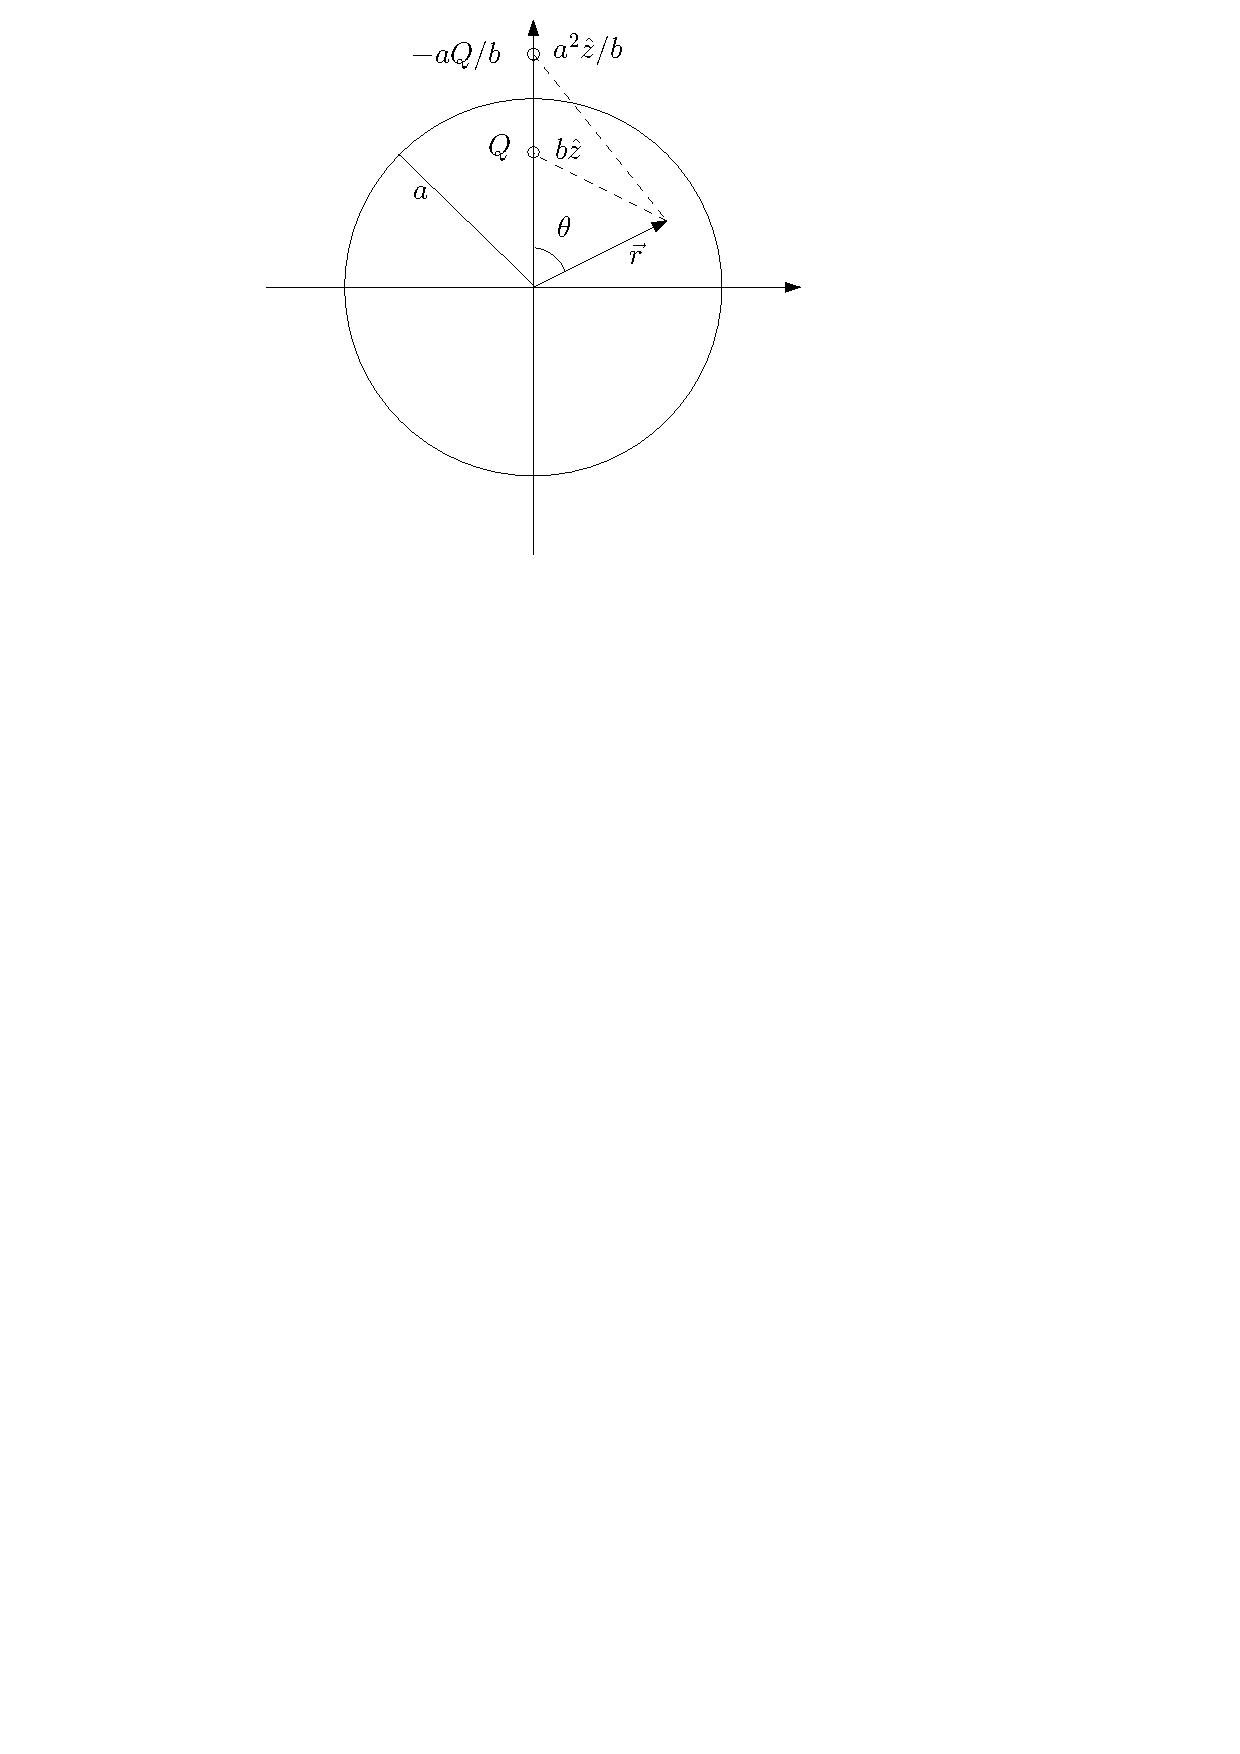
\includegraphics[width=0.5\linewidth]{fig-09-diffekv-veckanstal-spegling/spegling.pdf}}

\vspace{6mm}


Avstånden (streckade linjer i figuren) blir
\begin{align}
\left| \vec{r} - b\hat{z} \right| &= \sqrt{ r^2 + b^2 - 2 b r \cos\theta} \nonumber \\
\left| \vec{r} - \frac{a^2}{b}\hat{z} \right| &= \sqrt{ r^2 + \frac{a^4}{b^2} - 2 \frac{a^2}{b} r\cos\theta}
\end{align}

och lösningen är alltså 
$$
\phi(\vec{r}) = \frac{Q}{4\pi\epsilon_0} \left[ \frac{1}{\sqrt{r^2 + b^2 - 2 b r \cos\theta}} - \frac{a}{b} \frac{1}{\sqrt{r^2 + \frac{a^4}{b^2} - 2 \frac{a^2}{b} r\cos\theta}}\right].
$$
Vid radien $r=a$ kan vi skriva den andra termens nämnare $\sqrt{ \frac{a^2}{b^2} (b^2 + a^2 - 2 a b \cos\theta ) }$. Notera därför att denna lösning uppfyller det givna randvillkoret $\phi = 0$ på sfärens yta $r=a$.

Ytladdningsfördelningen ges av $\epsilon_0 \left. \hat{r} \cdot \left( \vec{E}^+ - \vec{E}^- \right) \right|_{r=a}$. Eftersom potentialen var noll utanför sfären blir $\sigma = -\epsilon_0 {E_r}^-$. Vi behöver alltså den radiella komponenten av det elektriska fältet
$$
E_r(\vec{r}) = -\frac{\partial \phi}{\partial r} = \frac{Q}{4\pi\epsilon_0} \left[ \frac{r - b\cos\theta}{(r^2 + b^2 - 2 b r\cos\theta)^{3/2}} - \frac{a}{b} \frac{r - \frac{a^2}{b}\cos\theta}{(r^2 + \frac{a^4}{b^2} - 2 \frac{a^2}{b}r\cos\theta)^{3/2}} \right].
$$
Vid radien $r=a$ får vi
$$
\left. E_r \right|_{r=a} = \frac{Q}{4\pi\epsilon_0} \frac{a^2 - b^2}{a(a^2 + b^2 - 2ab\cos\theta)^{3/2}}.
$$

Alltså får vi ytladdningen
$$
\sigma = -\epsilon_0 \left. E_r \right|_{r=a} = -\frac{Q}{4 \pi} \frac{a^2 - b^2}{a \left( a^2 + b^2 - 2 a b \cos\theta \right)^{3/2}}.
$$
Den totala laddningen på sfärens yta ($\mbox{d}S = a^2 \sin\theta \mbox{d}\varphi \mbox{d}\theta$) fås nu genom att integrera
\begin{align}
Q' &= \int_{r=a} \sigma \mbox{d}S = -\frac{Q}{4\pi} \frac{a^2-b^2}{a} \int_{\varphi=0}^{2\pi} a^2 \mbox{d}\varphi \int_{\theta=0}^\pi \frac{\sin\theta \mbox{d}\theta}{\left( a^2 + b^2 - 2 a b \cos\theta \right)^{3/2}} \nonumber \\
&= \left\{ \begin{array}{ll}
\cos\theta = t & \Rightarrow \mbox{d}t = -\sin\theta \mbox{d}\theta \\
\theta \in [0,\pi] & \Rightarrow t \in [1,-1] \\
\end{array} \right\} = - \frac{Q}{2} (a^2 - b^2) a \int_{-1}^1 \frac{\mbox{d}t} {\left( a^2 + b^2 - 2 a b t \right)^{3/2}} \nonumber \\
& = - \frac{Q}{2} (a^2 - b^2) a \left[ \frac{1}{ab} \frac{1}{\left( a^2 + b^2 - 2 a b t \right)^{1/2}} \right]_{-1}^1 = - \frac{Q}{2} \frac{(a^2 - b^2)}{b} \left[ \frac{1}{a-b} - \frac{1}{a+b} \right] \nonumber \\
& = - \frac{Q}{2} \frac{(a^2 - b^2)}{b} \frac{a + b - (a - b)}{a^2 - b^2} = -Q.
\end{align}

% --- end solution of exercise ---

% Closing remarks for this Exercise

\paragraph{Remarks.}
Uppgiften illustrerar speglingsmetoden för att lösa Poissons ekvation i specifika geometrier. Notera speciellt hur den införda speglingsladdningen ligger utanför det relevanta området, men ändå ger ett bidrag till fältet. Potentialen kan tecknas direkt utifrån uppgiften, men det kan vara en god idé att faktiskt skriva ner Greensfunktionen och utföra volymsintegralen med en laddningsfördelning som motsvarar en punktladdning i punkten $b \hat{z}$.


\end{doconceexercise}
% --- end exercise ---


% ------------------- end of main content ---------------

\end{document}

